
\section{Quantum Gate Model}
\label{sec:qgmc}
In diesem Kapitel werden wir die im Titel der Arbeit angesprochene Idealumsetzung näher betrachten. In der derzeitigen NISQ-Ära (Stand 22.06.2021) entspricht dies leider noch überhaupt nicht der Wirklichkeit, hierzu folgt im Kapitel 3 dann mehr.
\subsection{Theoretische Grundlagen}
Bevor wir uns der tatsächlichen Umsetzung des Quantum Gate Models (QGM) widmen, sollten wir uns zunächst einmal der benötigten Grundlagen hierfür vertraut machen.\\
Grundlage des QGM ist die Quantenmechanik. Diese nanophysikalische Theorie entsprang der sogenannten Kopenhagener Interpretation von N. Bohr und W. Heisenberg 1927\cite[Seiten 108-111]{KopoBaker}.
Das zentrale Objekt hierbei ist eine sogenannte Wellenfunktion \(\Psi\)(\(\mathbf{r}\),t)\(\in \mathcal{H}(\mathbb{C}^n)\) zur Beschreibung aller Informationen eines Systems und als Lösung der Schrödingergleichung (Postulat von E. Schrödinger 1926), die wie folgt lautet\cite[Seite 22]{GriffithsQuantumMechanics}:
\begin{equation}
i \hbar \frac{\partial}{\partial t}\Psi(\mathbf{r},t) = \hat H \Psi(\mathbf{r},t)
\end{equation}
Hierbei seien \(i\) die imaginäre Einheit, \(\hbar\) das plank'sche Wirkungsquantum, \(\mathbf{r}\) der (mehrdimensionale) Ort und \( \hat H\) der selbst-adjungierte Hamiltonoperator (oder auch Energieoperator).\\
Nun lässt sich die Wellenfunktion mithilfe ihrer Eigenzustände darstellen. Diese werden meistens mit \(\Psi_n\) bezeichnet. Daraus resultiert die für die Quantenmechanik berühmte Dirac-Notation (nach P. Dirac)\cite[Seite 154]{GriffithsQuantumMechanics}:
\begin{align}
\ket{\Psi} &=: \begin{bmatrix}
           \Psi_{1} \\
           \Psi_{2} \\
           \vdots \\
           \Psi_{n}
         \end{bmatrix}
\text{("Ket"), } 
\bra{\Psi} =: (\Psi_{1}^* \,\Psi_{2}^*\, \cdot\cdot\cdot \Psi_{n}^*) \text{ ("Bra")}
\end{align}
Der Umstieg von klassischer auf quantenmechanische Physik wirkt sich natürlich auch auf das zugrundeliegende System aus. So werden nicht mehr wie bei klassischen Binärrechnern Bits verwendet, die entweder den Zustand 0 oder 1 annehmen können.
Vielmehr werden nun sogenannte Quantenbits - oder kurz Qubits - eingesetzt. Ein Qubit kann mehr als nur die Zustände 0 und 1 annehmen. Es kann auch die überlagerten Zustände annehmen, genauer\cite[Seite 20]{QuantumComputingHomeister}:
\begin{equation}
\text{Seien }\alpha, \beta \in \mathbb{C}.\text{ Dann gilt: }\ket{\Psi} = \alpha \cdot \ket{0} + \beta \cdot \ket{1} \text{ mit }|\alpha|^2 + |\beta|^2 = 1.
\end{equation}
Die Überlagerung dieser Zustände wird auch Superpostion genannt.\\
Erfolgt nun eine Messung des Qubits, so kollabiert die Wellenfunktion und das Qubit befindet sich mit Wahrscheinlichkeit \(|\alpha|^2\) im Zustand \(\ket{0}\) und \(|\beta|^2\) im Zustand \(\ket{1}\)\cite[Seite 20]{QuantumComputingHomeister}.\\

Wie im klassischen Sinne, werden Qubits natürlich auch in Gattern verbaut. Diese Gatter nennt man Quantum Gates. Grundlage dieser Gatter sind Matrizen M \(\in\) U(n) (Unitary Group).\\
\newpage
Wichtige Beispiele mit zugehörigem Gatter:\\
\begin{figure}[!htb]
\floatbox[{\capbeside\thisfloatsetup{capbesideposition={right},capbesidewidth=4cm}}]{figure}[\FBwidth]
{\caption{Die wichtigsten Gatter in einer Übersicht \cite{Gates}}\label{fig:test}}
{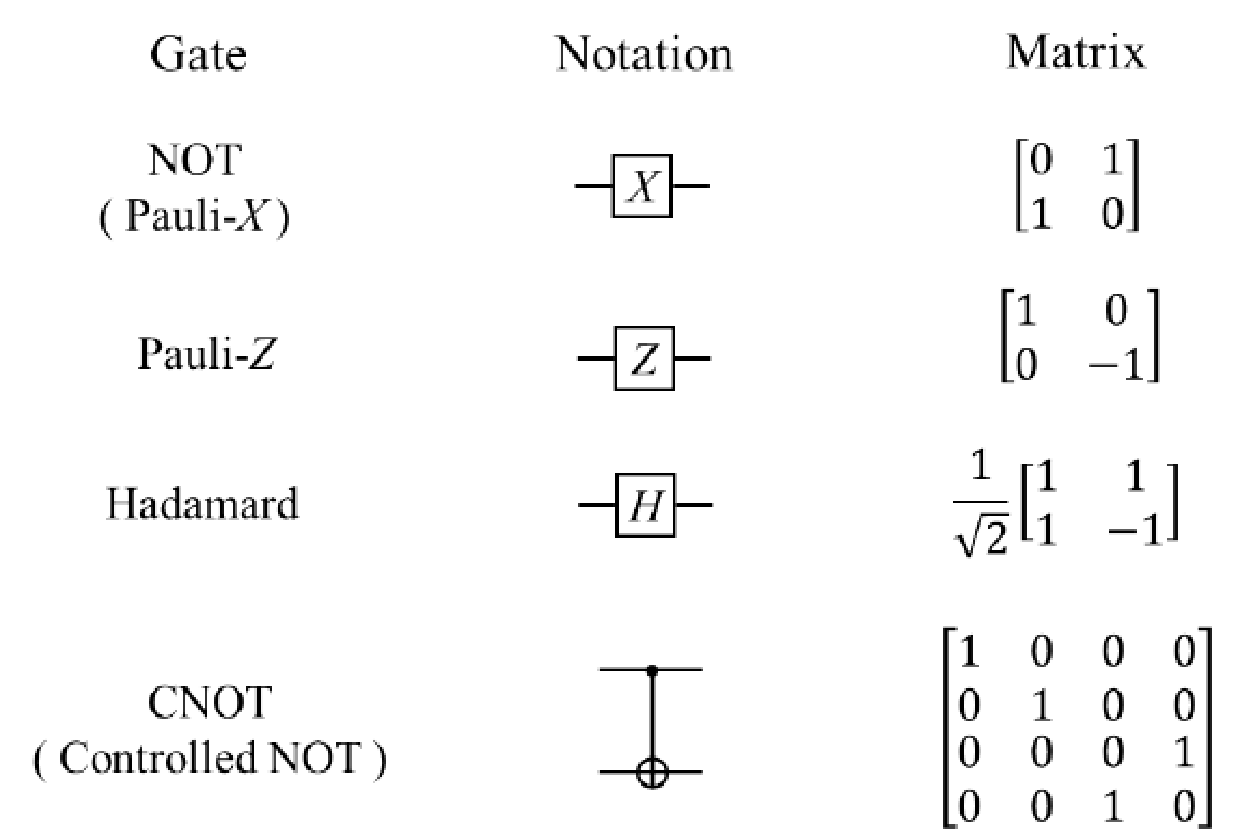
\includegraphics[width=11cm]{QML/images/gates.pdf}}
\end{figure}\\

Setzen wir nun mehrere Quantum Gates zusammen, erhalten wir - ähnlich wie im klassischen Sinne - sogenannte Quantenregister. Mathematisch kann man eine merkwürdige Eigenschaft dieser Quantenregister sehr schnell herleiten: Die sogenannte Verschränkung. Zunächst sei diese folgendermaßen definiert\cite[Seiten 53,55]{QuantumComputingHomeister}:\\

Sei $\ket{\Psi}$ der Zustand eines Quantenregisters mit n Bits (also folglich n Eigenzuständen), \(n \in \mathbb{N}\). Dieser Zustand heißt genau dann unverschränkt, wenn gilt:\\
\begin{equation}
    \ket{\Psi} = \ket{\Psi_{n-1}} \otimes \ket{\Psi_{n-2}} \otimes ... \otimes \ket{\Psi_{0}}
\end{equation}
Hierbei sei $\otimes$ logischerweise das Tensorprodukt zwischen den Eigenzuständen.\\
Der Zustand heißt folglich genau dann verschränkt, wenn keine solche Partitionierung existiert.\\
Merkwürdig erscheint hierbei nun intuitiv gesehen, dass eine Änderung eines Bits die Messung eines anderen Bits beinflusst, da die Eigenzustände miteinander verschränkt sind.\\

Zuletzt betrachten wir noch die wohl berümteste und gleichzeitig zentrale Folgerung aus der Quantenmechanik: Die Heisenbergsche Unschärferelation. Diese lautet wie folgt\cite{HeisenbergPascuzzo}:\\
\begin{equation}
\begin{split}
\text{Es seien } f,tf(t), \omega \hat{f}(\omega) \in L^2(\mathbb{R}).\text{ Dann gilt: }
(\int\limits_{-\infty}^{+\infty} t^2|f(t)|^2 dt)(\int\limits_{-\infty}^{+\infty} \omega^2|\hat{f}(\omega)|^2 d\omega)\ge \frac{A}{4B}(\int\limits_{-\infty}^{+\infty} |f(t)|^2 dt)^2
\end{split}
\end{equation}
\textbf{Anmerkung:} \(L^2\) steht hierbei für den 2-dimensionalen Lebesgue-Raum, $\hat{f}(\omega)$ für die übliche\linebreak Fourier-Transformation Notation von f(t). Zudem gelte AB=$\frac{1}{2\pi}$.\\
Intuitiv bedeutet dies: Zwei komplementäre Eigenschaften eines Systems sind nicht beliebig genau messbar. Ein Beispiel sind Ort und Impuls, die bei Messung des einen die andere Größe jeweils entscheidend beeinflusst.\\
Dies widerspricht schon deutlich der klassischen menschlichen Vorstellung. Die Folge ist, dass das logisch intuitive Verständnis nahezu komplett verloren geht.\\
\subsection{Praktische Idealumsetzung}
Nachdem wir uns der wichtigsten mathematischen Grundlagen vertraut gemacht haben, widmen wir uns in
diesem Kapitel nun der Umsetzung im QML. Bisher konnte nur für Algorithmen, die auf dem Grover-Algorithmus (GA) basieren, Quantenvorteile bewiesen werden\cite{PartialQuantumSearchGrover}. Mit Quantenvorteilen sind hierbei\linebreak Geschwindigkeits-/Effizienzvorteile gegenüber vergleichbaren Machine Learning (ML) Algorithmen auf klassischen Binärrechnern gemeint.\\
Erwähnt sei hier noch ein weiterer bekannter Algorithmus, der sogenannte Shor-Algorithmus, der Fourier-Transformationen in $\mathcal{O}(n^3)$ durchführen kann\cite{ShorAlgorithm}. Wir verbleiben bei dem Verweis hier und fokusieren uns auf den GA.\\

Bevor wir zwei Anwendungen basierend auf dem GA näher betrachten, sollten wir uns logischerweise dem GA selbst erst einmal vertraut machen:\\

\begin{algorithm}
\caption{Grover Algorithmus\cite{FastQuantumAlgorithmGrover}}
\begin{algorithmic}[1]
\Procedure{Grover Algorithmus}{$N,S,i,j$}
\State $\text{initialisiere das System durch die Verteilung} (\frac{1}{\sqrt{N}}$, $\frac{1}{\sqrt{N}}$, ... , $\frac{1}{\sqrt{N}}) \text{ für jeden der }N \in \mathbb{N} \text{ Zustände}$
\While{O($\sqrt{N}$)}
\State $\text{Für Zustand S:}$
\If{Cond(S) = 1}
\State $\text{rotiere die Phase um } \pi \text{ Radianten}$
\ElsIf{Cond(S) = 0}
\State $\text{System bleibt unverändert}$
\State $\text{Wende die Diffusions-Transformation D an, die definiert ist als:}$
\State $D_{ij} = \frac{2}{N} \text{ falls } i \neq j$, $D_{ii} = -1 + \frac{2}{N}$
\EndIf
\EndWhile
\State Frage den resultierenden Zustand ab:
\If{Cond($\text{S}_{\nu}$) = 1}
\State $\exists! \text{S}_{\nu}$, sodass $\text{S}_{\nu}$ der Endzustand ist mit Wahrscheinlichkeit $\frac{1}{2}$
\EndIf
\EndProcedure
\end{algorithmic}
\end{algorithm}
Die Idee hinter diesem Algorithmus ist das Prinzip der sogenannten 'Amplitudenverstärkung'. Dabei ist letztere eine Verallgemeinerung des GA\cite{QuantumAmplitudeAmplificationBrassard}.\\
Für ein konkretes, praxisorientiertes Beispiel verweisen wir an dieser Stelle auf \cite{GroverExample}.
\newpage
\subsubsection{Der Viterbi Algorithmus}
Im Folgenden lernen wir nun noch 2 konkrete Beispiele kennen, wie QML aussehen würde, wenn die nötige Technik hierfür bereitsteht.\\

Für den Viterbi Algorithmus (VA) als erstes Beispiel gibt es sowohl eine klassische, als auch eine quantenmechanische Version. Letztere stellt hierbei eine Verbesserung insofern dar, als dass die klassische Suche nach dem maximalen Wert (Max) durch eine quantenmechanische Version (QuantumMax) ersetzt wird. QuantumMax nutzt hierbei einen Algorithmus, der eine QuantumSearch benutzt, die widerum auf dem GA aufbaut\cite{RuntimeOptiBishwas}.\\
Konkret sieht der Algorithmus dann wie folgt aus:

\begin{algorithm}
\caption{Quantum Viterbi Algorithm \cite{RuntimeOptiBishwas2}}
\begin{algorithmic}[1]
\Procedure{QuantumViterbi}{$O,S,\Pi,Y,A,B$}
\For{Zustand i=1,2,...,K}
\State $\pi_i \cdot B_{iy_1} \to \phi_1[i,1]$
\State $0 \to \phi_1[i,1]$
\EndFor
\For{Observable j=2,3,...,$\phi$}
\For{Zustand i = 1,2,...,K}
\State $\textit{QuantumMax}(\phi_1[k,j-1] \cdot A_{ki} \cdot B_{iy_j},K)[0] \to \phi_1[i,j]$
\State $\textit{QuantumMax}(\phi_1[k,j-1] \cdot A_{ki} \cdot B_{iy_j},K)[0] \to \phi_2[i,j]$
\EndFor
\EndFor
\State $QuantumMax(\phi_1[k,\phi],K)[1] \to z_{\phi}$
\State $s_{z\phi} \to x_{\phi}$
\For{j=$\phi,\phi - 1, ..., 2$}
\State $\phi_2[z_j,j] \to z_{j-1}$
\State $s_{z_{j-1}} \to x_{j-1}$
\EndFor
\State $x_{\phi} \to X$
\State $\textbf{return }X$
\EndProcedure
\end{algorithmic}
\end{algorithm}
Hierbei stehen X für die Menge an hidden states (aus dem Hidden Markov Modell), S für die Menge an Zuständen, Y die Menge an Observablen, die mit dem Oberservablenraum O generiert werden, $\Pi$ für die Menge an Initialwahrscheinlichkeiten, A ist eine Übergangsmatrix, B eine Emissionsmatrix. $\phi_n[i,j]$ von $\phi_n, n \in \mathbb{N}$ speichert die Wahrscheinlichkeit des günstigsten Pfades. Alle Kleinbuchstaben wie x sind stellvertretend für Elemente der eben aufgezählten Mengen\cite{RuntimeOptiBishwas2}.
\newpage
\subsubsection{Quantenbasiertes Reinforcement Learning}
Um die Idee hinter dem quantenbasierten Reinforcement Learning (QRL) verstehen zu können, sollten wir uns erst einmal klassischem RL kurz widmen. Die Grundidee ist hierbei, dass der Software-Agent eine eigene sequentielle Entscheidungsfindung besitzt, indem verschiedene Belohnungen vergeben werden - positive wie negative\cite{IntroDeepReinfLavet}.
Für die Optimierung des klassischen Ansatzes wird im QRL nun der GA wieder genutzt. Im Detail sieht das dann folgendermaßen aus:\\

\begin{algorithm}
\caption{Quantum Reinforcement Learning \cite{QuantumReinfDong}}
\begin{algorithmic}[1]
\Procedure{QRL}{$a,s,r$}
\State $\text{Initialisiere }\ket{s^{(m)}} = \sum_{s=00\cdot\cdot0}^{11\cdot\cdot1} C_s \ket{s}, f(s) = \ket{a_s^{(n)}} = \sum_{s=00\cdot\cdot0}^{11\cdot\cdot1} C_a \ket{a} \text{ und V(s) beliebig}$
\For{Zustände $\ket{s}$ in $\ket{s^{(m)}} = \sum_{s=00\cdot\cdot0}^{11\cdot\cdot1} C_s \ket{s}$}
\State $\text{Beobachte f(s) } = \ket{a_s^{(n)}} \text{ und erhalte }\ket{a}$
\State $\text{Wirke }\ket{a},\text{beobachte den nächsten Zustand }\ket{s'},\text{ erhalte r, dann:}$
\State $\text{(a) Aktualisiere den Zustandswert: V(s)}\leftarrow \text{V(s) + }\alpha(r + \gamma\text{V(s') - V(s))}$
\State $\text{(b) Aktualisiere die Wahrscheinlichkeitsamplituden:}$
\Repeat
\State $U_{Grov} \ket{a_s^{(n)}} = U_{a_0^{(n)}}U_a\ket{a_s^{(n)}}$
\Until{$\#U_{Grov} = L$}
\EndFor
\State $\textbf{Until } \forall \text{Zustände s: } |\Delta\text{ V(s)}|\le \epsilon$
\EndProcedure
\end{algorithmic}
\end{algorithm}
Hierbei seien $\text{U}_{Grov}$ eine Grover-Iteration (U ist ein Operator), V(s) das Bild der Zustände (also die Zustandswerte), L=int(k(r+V(s'))) (int(x) gibt den ganzzahligen Anteil von x zurück), C die Wahrscheinlichkeitsamplituden.
